% Number 350
% CAPMA Algebra Units
% Car slowing up hill
% JG

% Watermark
\AddToShipoutPicture*{\BackgroundPic}

\addtocounter {ProbNum} {1}

%\begin{floatingfigure}[r]{.3\textwidth}
%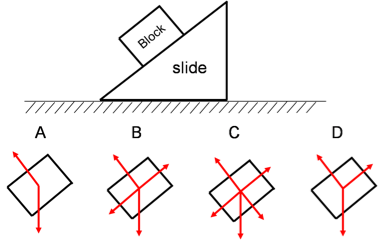
\includegraphics[scale=.4]{/Users/jgates/desktop/latex/pics/incline3.png}
%\end{floatingfigure}
 
{\bf \Large{\arabic{ProbNum}}} A car that is moving ${30~\tfrac{m}{s}}$ runs out of gas while driving up a hill.  The car comes to a stop 150 meters further up the hill than the point at which it ran out of gas. 

\begin{center}
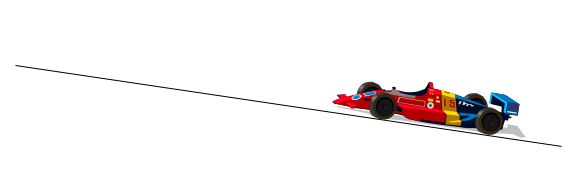
\includegraphics[scale=.6]{/Users/jgates/desktop/latex/pics/caruphill.png}
\end{center}

\bigskip  How long, after running out of gas, did it take for the car to come to a stop?  Also describe, in words, the direction of the acceleration. Draw a kinematics diagram as part of your solution.


\vfill
\newpage
